{Terminata la breve parentesi teorica introduttiva,  si procede in questo capitolo alla presentazione
dell'impostazione pratica che si è voluto dare alle sperimentazioni condotte. La struttura secondo cui
saranno esposte le informazioni nei seguenti paragrafi ricalca la partizione logica alla base del codice
sviluppato, pragmaticamente diviso in quattro moduli tra loro indipendenti:}

\begin{itemize}
\item generazione dei grafi
\item generazione delle istanze di problemi MIP
\item risoluzione delle istanze di problemi MIP
\item estrazione ed analisi dei dati
\end{itemize}

\section{Generazione di grafi}
L'iniziale problema che è stato necessario affrontare nello svolgimento di questo lavoro è stata la 
generazione automatica e pseudo-casuale di grafi, indispensabile al fine di ottenere un numero sufficiente di 
istanze da cui estrarre informazioni statisticamente rilevanti. Quello della generazione di grafi pseudo-casuali è un problema noto in letteratura, in quanto in numerosi ambiti di ricerca, che spaziano dalla biologia 
molecolare allo studio delle reti di calcolatori, si rende necessaria la generazione casuale di queste strutture 
dati nello studio delle realtà di loro interesse. 
Di conseguenza, nel corso degli ultimi decenni sono stati molti i metodi proposti dalla comunità scientifica al 
fine di affrontare il problema. Tra questi ne sono stati selezionati quattro, sulla base delle proprietà e delle 
caratteristiche particolari di ciascuno di essi.  

L'implementazione dei metodi per la generazione casuale di grafi è stata fatta utilizzando NetworkX, una libreria stabile e flessibile sviluppata appositamente per lo studio e la rappresentazione di grafi in Python \cite{networkx}. NetworkX offre, oltre alla possibilità di rappresentazione, diversi algoritmi per lo studio delle proprietà e il calcolo di misure in specifiche istanze di grafi. 

\subsection{Modello di Erdős–Rényi}
Il modello di Erdős–Rényi è un modello per la generazione di grafi casuali, detti grafi Erdős–Rényi (\textsl{ER}) o binomiali, introdotto per la prima volta nel 1959 dai matematici ungheresi Paul Erdős e Alfréd Rényi \cite{erdos59a}. 
Nella formulazione $G(n,p)$ del modello,  un grafo di $n$ nodi viene costruito secondo un procedimento iterativo, in cui ogni arco tra due nodi del grafo viene formato indipendentemente dagli altri con una probabilità fissa $p$.  

\theoremstyle{definition}
\newtheorem{definizione}{Definizione}
\begin{definizione}
Un grafo ER, anche detto $G(n,p)$, è un grafo (N,G) con $N={1,2,\dots n}$ e in cui la matrice delle adiacenze G = $(g_{ij}$ è tale per cui, per ogni coppia di nodi distinti $i$ e $j$, a probabilità che $g_{ij} = 1$ è $P(g_{ij}=1)=p,$, con $p \in [0,1]$ fissato. 
\end{definizione}

I parametri di questo modello sono quindi due, il numero di nodi del grafo $n$ e la probabilità di generazione di ogni arco $p$.  A parità di parametri, i grafi che si possono ottenere sono in ogni caso molti, come mostrato in Figura (\ref{fig:gnpes}). 

\begin{figure}[h!]
     \centering
     \begin{subfigure}[b]{0.25\textwidth}
         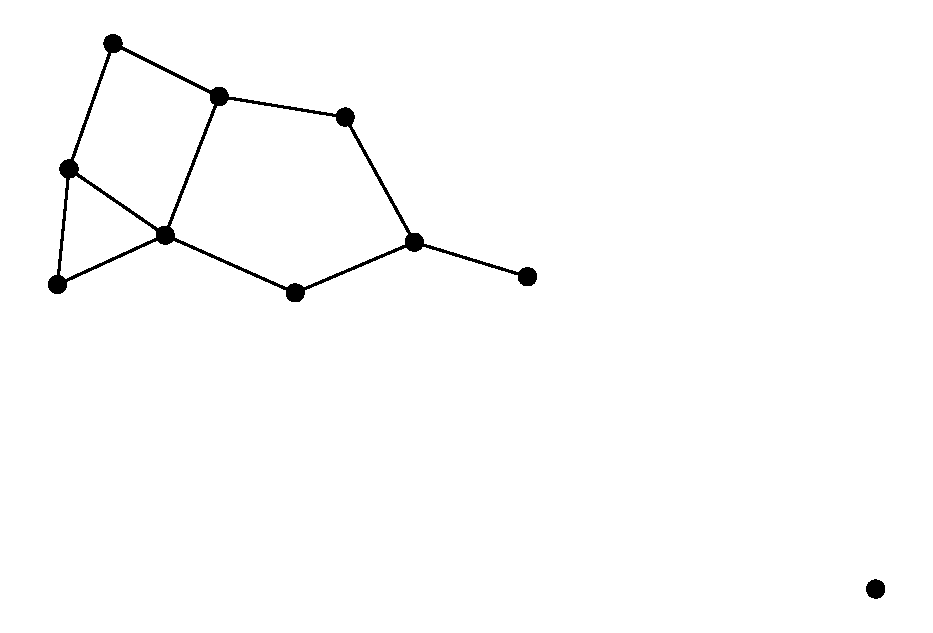
\includegraphics[width=\columnwidth]{images/gnpes0.eps}
     \end{subfigure}
     \hspace{0.8em}
     \begin{subfigure}[b]{0.25\textwidth}
         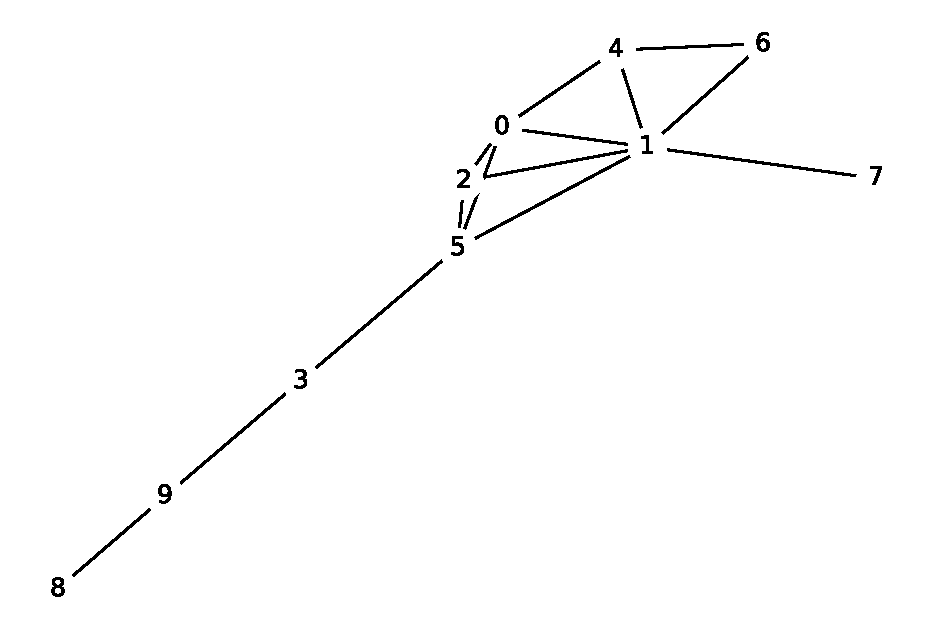
\includegraphics[width=\columnwidth]{images/gnpes1.eps}
     \end{subfigure}
     \hspace{0.8em}
     \begin{subfigure}[b]{0.25\textwidth}
         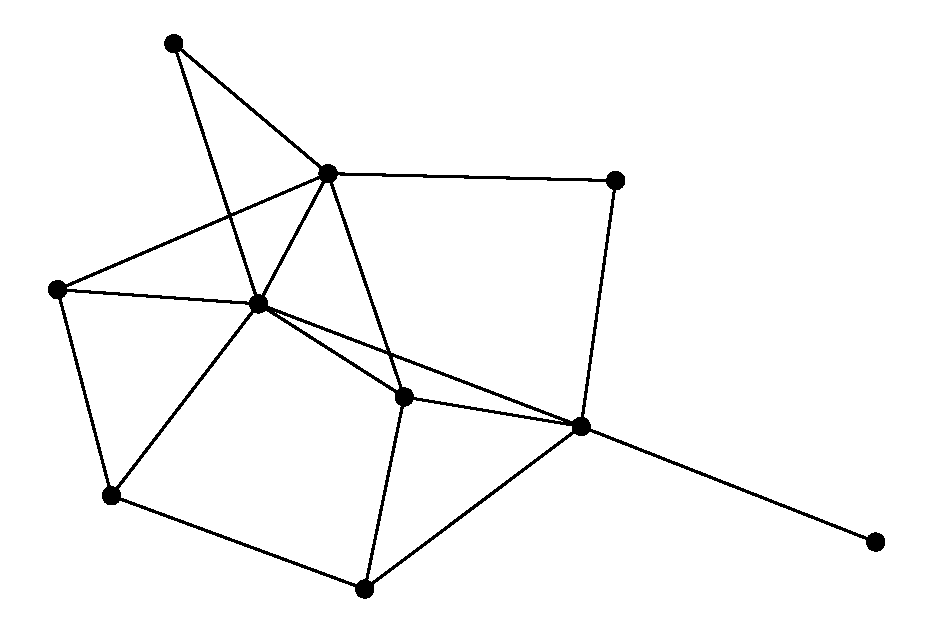
\includegraphics[width=\columnwidth]{images/gnpes2.eps}
     \end{subfigure}
        \caption{Diversi grafi $G(n,p)$ generati a partire dagli stessi parametri $n=10$ e $p=0.3$ con la libreria NetworkX e visualizzati graficamente con l'ausilio di un'altra libreria Python, Matplotlib \cite{Hunter2007}.}
        \label{fig:gnpes}
\end{figure}

\begin{algorithm}
\SetAlgoLined
\KwIn{numero di nodi $n$ e probabilità di generazione di ogni arco $p$}
 inizializza il grafo vuoto $G$\;
 aggiungi i nodi $1 \dots n$ a $G$\;
 \ForEach{{\upshape arco} e {\upshape tra due nodi del grafo}}{
 	$rand$ = numero casuale $\in [0,1]$\;
 	\If{rand $>$ p} {
 		aggiungi $e$ a $G$\;
 	}
 }
 \Return{$G$}
 \caption{Generazione di un grafo di Erdős–Rényi}
 \label{alg:gnp}
\end{algorithm}

Il metodo di NetworkX utilizzato nella generazione di questa tipologia di grafi è \linebreak
\texttt{gnp\_random\_graph(n, p, seed)}, che restituisce un'istanza di grafo binomiale di dimensione \texttt{n} in cui gli archi hanno probabilità di essere generati pari a \texttt{p}, mentre il parametro \texttt{seed} regola il comportamento pseudo-casuale, in modo tale da permettere la riproducibilità degli esperimenti. Lo pseudo-codice dell'algoritmo che gestisce la generazione di questa tipologia di grafi è riportato in Algoritmo (\ref{alg:gnp}).

\subsection{Generazione di grafi regolari}

\subsection{Modello di Watts-Strogatz}
Il modello di Watts-Strogatz è un modello per la generazione di grafi casuali presentato nel 1998 da Duncan J. Watts e Steven Strogatz \cite{watts_collective_1998}, la cui caratteristica principale risiede nel possedere proprietà \textit{small-world}, come ad esempio alto coefficiente di clustering globale e bassa lunghezza media dei cammini all'interno del grafo. 

Il concetto di small-world venne introdotto per la prima volta nel 1967 dallo psicologo statunitense Stanley Milgram nella sua serie di esperimenti mirata ad esaminare la lunghezza media dei percorsi delle reti sociali tra residenti negli Stati Uniti, in cui ipotizzava per l'appunto un "\textit{piccolo mondo}", composto da una rete di collegamenti tra persone relativamente breve \cite{milgram_small-world_1967}.  Sulla base di queste considerazioni 



\subsection{Modello di Barabási-Albert}







